\subsubsection{Ý tưởng}
Selection Sort là thuật toán sắp xếp dựa trên so sánh. Thuật toán này sắp xếp một mảng bằng cách chọn đi chọn lại phần tử nhỏ nhất (hoặc lớn nhất) từ phần chưa được sắp xếp và hoán đổi nó với phần tử chưa được sắp xếp đầu tiên. Quá trình này tiếp tục cho đến khi toàn bộ mảng được sắp xếp. \cite{brown2021selection}
\subsubsection{Mã giả}

\begin{algorithm}[H]
    \caption{Selection Sort}
    \begin{algorithmic}[1]
    \Procedure{SelectionSort}{$arr, n$}
        \State \textbf{Input:} Mảng $arr$ gồm $n$ phần tử
        \State \textbf{Output:} Mảng $arr$ được sắp xếp
        
        \For {$i \gets 0$ \textbf{to} $n-1$}
            \State $minIdx \gets i$
            \For {$j \gets i+1$ \textbf{to} $n-1$}
                \If{$arr[j] < arr[minIdx]$}
                    \State $minIdx \gets j$
                \EndIf
            \EndFor
            \If{$minIdx \neq i$}
                \State \textbf{swap} $arr[i]$ \textbf{and} $arr[minIdx]$
            \EndIf
        \EndFor
    \EndProcedure
    \end{algorithmic}
    
\end{algorithm}
\newpage
\subsubsection{Ví dụ}
Giả sử chúng ta có mảng ban đầu: $[42, 17, 93, 58, 21, 76, 34]$. Dưới đây là các bước thực hiện Selection sort minh họa bằng hình ảnh:

\begin{figure}[H]
    \centering
    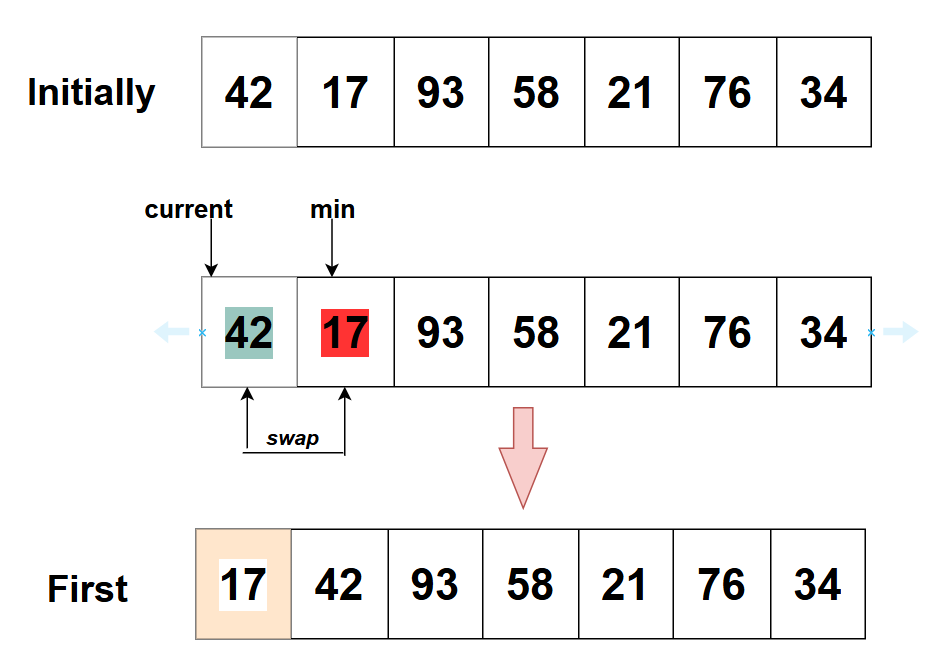
\includegraphics[width=0.7\textwidth]{img/selection sort/1.png}
    
\end{figure}

\begin{itemize}
\item Bắt đầu với phần tử đầu tiên(vị trí \textbf{curr}), chạy từ \textbf{curr} đến cuối mảng tìm phần tử nhỏ nhất (vị trí \textbf{min}) rồi hoán đổi hai phần tử ở vị trí \textbf{curr} và \textbf{min}. 
\begin{figure}[H]
    \centering
    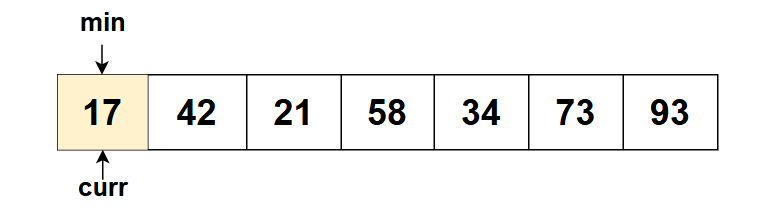
\includegraphics[width=0.7\textwidth]{img/selection sort/2.png}
    \caption{\textbf{curr} và \textbf{min} trùng nhau do 17 là phần tử nhỏ nhất}
\end{figure}

\begin{figure}[H]
    \centering
    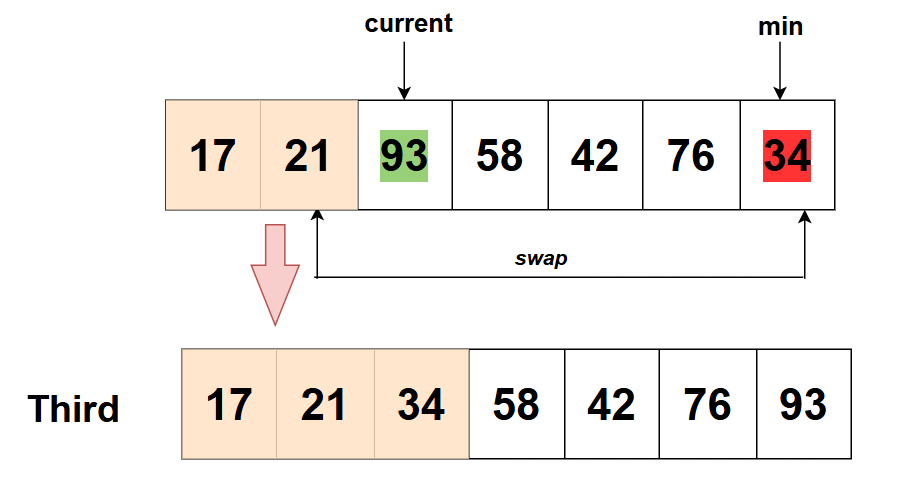
\includegraphics[width=0.7\textwidth]{img/selection sort/3.png}
    \caption{kết quả lần hoán vị đầu tiên.}
\end{figure}

\item Tiếp tục tăng \textbf{curr}, phần tử tiếp theo là vị trí \textbf{curr}, duyệt đến cuối mảng tìm phần tử nhỏ nhất (vị trí \textbf{min}) rồi hoán vị hai phần tử \textbf{curr} và \textbf{min}.

\begin{figure}[H]
    \centering
    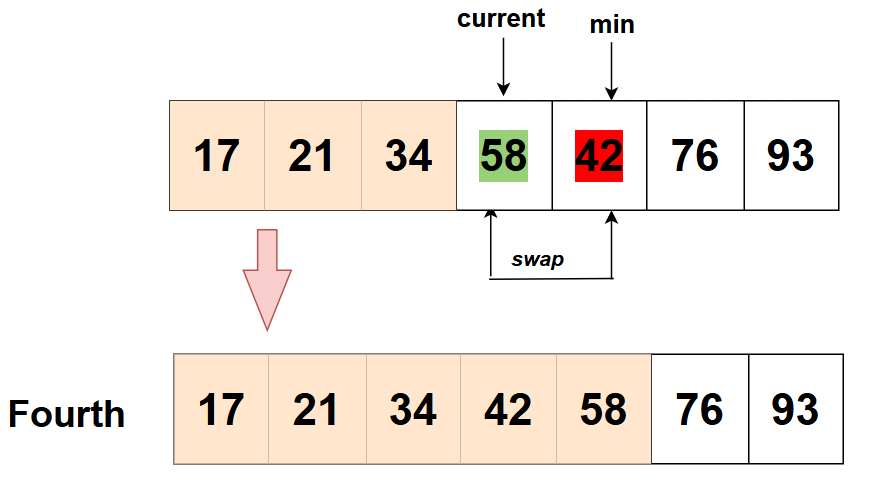
\includegraphics[width=0.7\textwidth]{img/selection sort/4.png}
    \caption{ta sẽ hoán đổi 42 và 21}
\end{figure}

\begin{figure}[H]
    \centering
    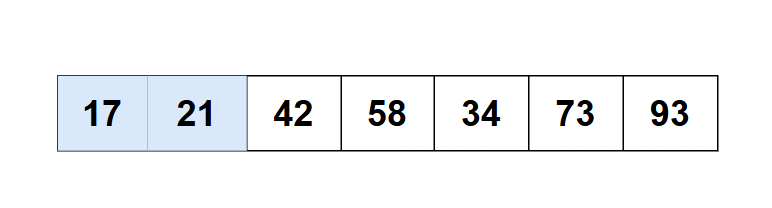
\includegraphics[width=0.7\textwidth]{img/selection sort/5.png}
    \caption{kết quả lần hoán vị thứ 2} 
\end{figure}

\item  Thực hiện tương tự cho đến khi mảng được sắp xếp.
\begin{figure}[H]
    \centering
    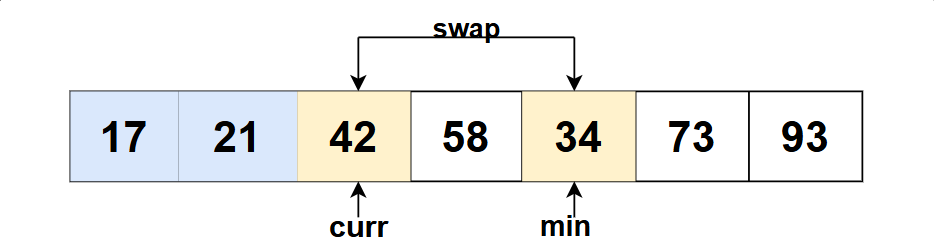
\includegraphics[width=0.7\textwidth]{img/selection sort/6.png} 
\end{figure}

\begin{figure}[H]
    \centering
    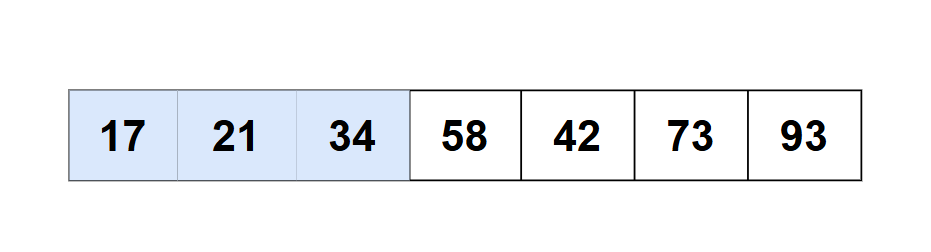
\includegraphics[width=0.7\textwidth]{img/selection sort/7.png} 
\end{figure}

\begin{figure}[H]
    \centering
    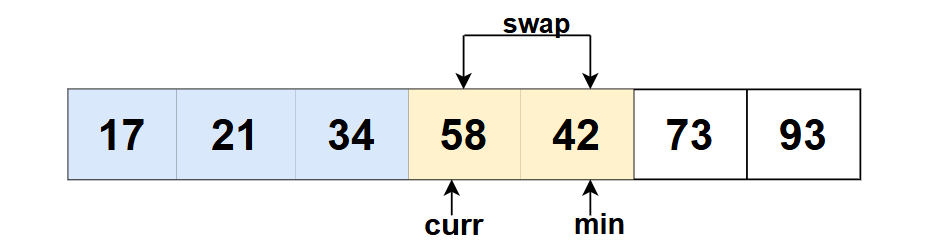
\includegraphics[width=0.7\textwidth]{img/selection sort/8.png} 
\end{figure}

\begin{figure}[H]
    \centering
    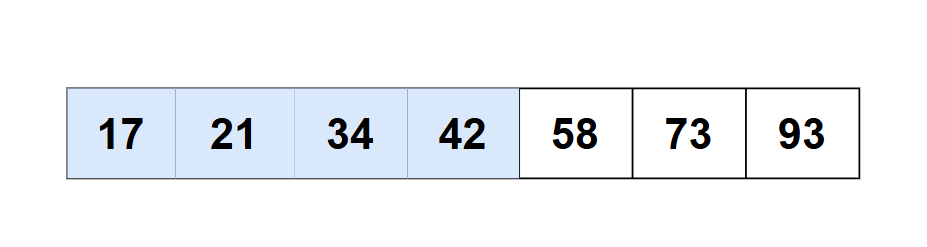
\includegraphics[width=0.7\textwidth]{img/selection sort/9.png} 
\end{figure}

\begin{figure}[H]
    \centering
    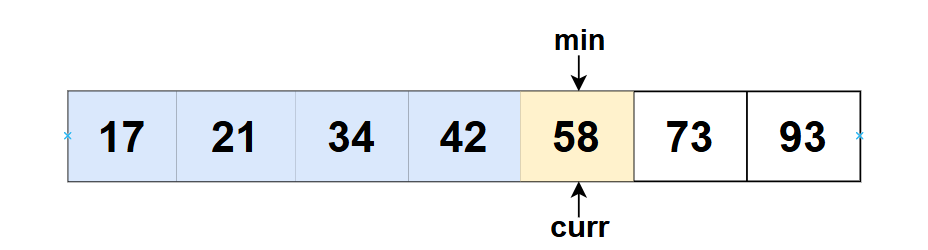
\includegraphics[width=0.7\textwidth]{img/selection sort/10.png} 
\end{figure}

\begin{figure}[H]
    \centering
    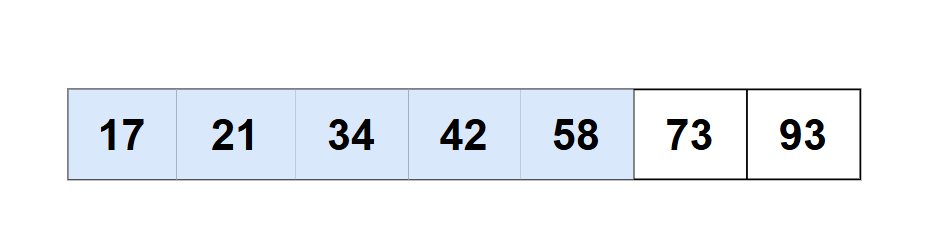
\includegraphics[width=0.7\textwidth]{img/selection sort/11.png} 
\end{figure}

\begin{figure}[H]
    \centering
    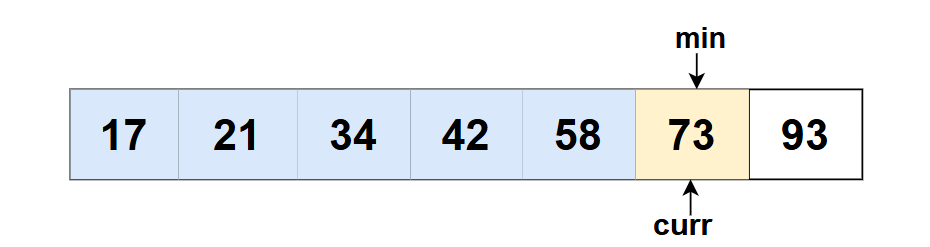
\includegraphics[width=0.7\textwidth]{img/selection sort/12.png} 
\end{figure}

\begin{figure}[H]
    \centering
    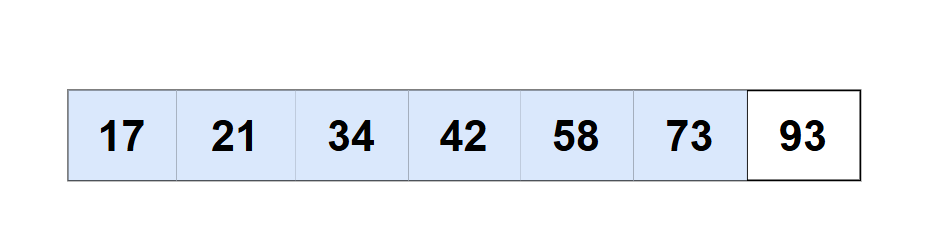
\includegraphics[width=0.7\textwidth]{img/selection sort/13.png} 
\end{figure}

\begin{figure}[H]
    \centering
    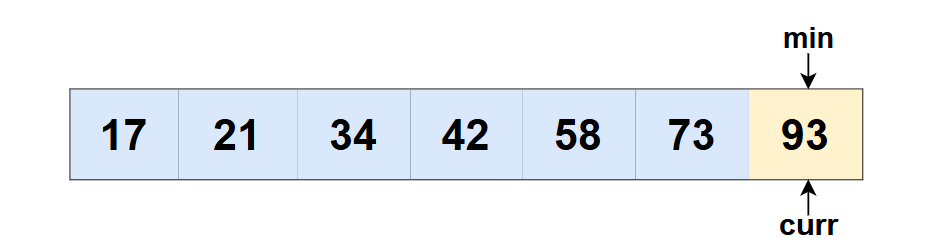
\includegraphics[width=0.7\textwidth]{img/selection sort/14.png} 
\end{figure}

\begin{figure}[H]
    \centering
    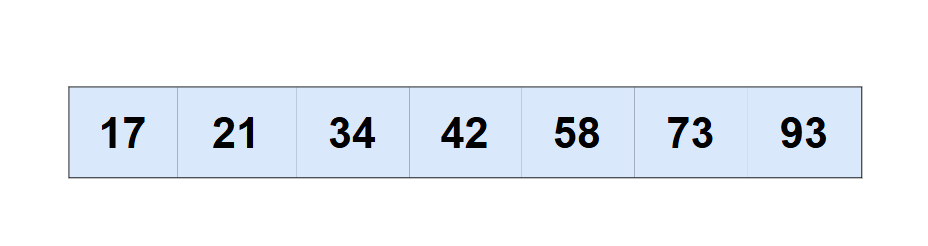
\includegraphics[width=0.7\textwidth]{img/selection sort/15.png} 
    \caption{Mảng đã được sắp xếp.}
\end{figure}


\end{itemize}

\subsubsection{{Độ phức tạp}}
\begin{itemize}
    \item[\textbf{--}] {Thời gian:}
    \begin{itemize}
        \item[$\bullet$] \textbf{Best Case:} \(\mathcal{O}(n^2)\), xảy ra ngay cả khi mảng đã được sắp xếp, vì thuật toán vẫn phải kiểm tra tất cả các phần tử để tìm giá trị nhỏ nhất trong mỗi lần lặp.
        \item[$\bullet$] \textbf{Average Case:} \(\mathcal{O}(n^2)\), trong trường hợp dữ liệu được phân bố ngẫu nhiên. Số lần so sánh và hoán đổi là cố định, không phụ thuộc vào cách dữ liệu được sắp xếp ban đầu.
        \item[$\bullet$] \textbf{Worst Case:} \(\mathcal{O}(n^2)\), xảy ra khi mảng ở trạng thái không sắp xếp. Thuật toán vẫn cần thực hiện \(n-1\) lần lặp, mỗi lần so sánh \(n-1\) phần tử còn lại.
    \end{itemize}
    \item[\textbf{--}] {Không gian:}
    \begin{itemize}
        \item[$\bullet$] Selection Sort là thuật toán \textbf{không yêu cầu bộ nhớ bổ sung} (\textbf{in-place}), vì nó chỉ sử dụng một biến phụ để lưu trữ giá trị tạm thời trong quá trình hoán đổi.
        \item[$\bullet$] Độ phức tạp bộ nhớ là:
        \[
        \mathcal{O}(1)
        \]
    \end{itemize}
    \item[\textbf{--}] {Tính ổn định:}
    \begin{itemize}
        \item[$\bullet$] Selection Sort là một thuật toán \textbf{không ổn định}. Khi hai phần tử có giá trị bằng nhau, vị trí tương đối của chúng có thể thay đổi sau quá trình hoán đổi.
    \end{itemize}
\end{itemize}